\chapter{Adversarial Examples and Training, GANs}

Deep learning has come quite far and as early as 2010s had neural networks that outperformed humans in several tasks. These networks were able to detect breeds of animals, faces to a degree of accuracy that humans cannot match. Now, we'll look at how easy it is to fool computers which is unusual given how well we've seen them perform. 

In adversarial classification, we are able to tweak images (such that it looks identitical to the human) so that the class of the image changes entirely.

This chapter is primarily from \href{https://www.youtube.com/watch?v=CIfsB_EYsVI}{this lecture of cs231n}. 

We aren't just barely crossing the decision boundary here though. We're leaping past it. 

\begin{figure}[h]
    \centering
    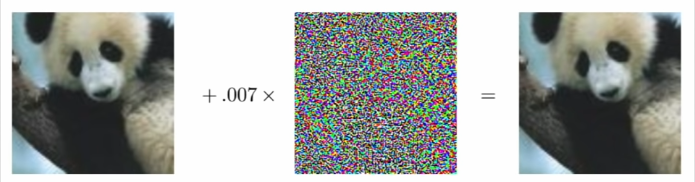
\includegraphics[width=12cm]{img/panda-adversary.png}
    \caption{Adversarial Example}
    \label{fig:panda}
\end{figure}

Here, the panda which was initially classified with a high degree of confidence was classified as another animal with an even higher degree of confidence later.

This vulnerability isn't limited to deep learning though. Even simple machine learning algorithms are susceptible to such behaviour. The lecture above shows how a linear softmax model was tricked such that the numbers (from the MNIST dataset) was tweaked and the trained model predicted the digital '9' to be any other digit. The tweaks did not substantially change the image at all. The same goes for logistic regressions and decision trees.

The initial explanation of this was that of overfitting, and the model fits the training set well and does randomly on the test set. But it was seen that this was not the case. The new idea was that of underfitting - like with linear models.

In fact, modern deep nets are like piecewise linear functions. Or rather, the mapping of the input to the output is linear - not parameters to output (which is non linear). This is interesting because with a linear model - there is a very high probability for a class assigned to points that aren't near our dataset to begin with. Hence, on such unseen data we are very confident about the class of our item. 

It's very easy for us to choose pertubations that choose the true class of an object. When making adversarial examples, we have to be careful to choose instances that retain the true class but give us a mismatch. It can be shown that for very small changes in our image vectors, the changes can have massive impact. 

\section{Fast Gradient Sign Method}

\textbf{Fast Gradient Sign Method} is a way to generate adversarial examples to attack a model by maximising a modified loss function that minimizes the distance between two images. The sign of the negative gradient of loss section determines how we want to change our image.

The adversarial examples were shown to exist in linear subspaces rather than in tiny groups which might have been the case with overfitting.   

To make things more interesting, it was shown that models in fact almost misclassify everything. That is, when you shift the input space for train and test data, the model performs very poorly. The lecturer goes on to show that for noise input, the CIFAR classifier gave high confidence for a lot of the images - one in four was considered to be an airplane - the lowest probability for any class. Ideally, we want to be able to know nothing or some abiguity from the classifier when fed noise. 

\section{Transferability}

 "Adversarial examples that affect one model often affect another model, even if the two models have different architectures or were trained on different training sets, so long as both models were trained to perform the same task.  An attacker may therefore  train  their  own substitute model,  craft  adversarial examples against the substitute, and transfer them to a victim model, with very little information about the victim" - from a \href{https://arxiv.org/pdf/1605.07277.pdf}{transferability of adversarial examples}.
 
 If the attacker doesn't have access to the target model itself - or have any knowledge of how it was obtained. We can train our own model and use that. If we don't have a training set, we can just send that training set as queries to the target model and use the label that is given. Making adversarial examples on our own model can then be found to transfer on the target dataset as well. 
 
 \textit{Optical illusions are like adversarial examples for humans} Perhaps this is indicative of a different learning method in our brains that the current deep learning methods.
 
 Training on adversarial examples has been found to reduce overfitting and helps generalize and improve the performance of models. Adversarial training introduces pertubations to the images to augment our training set. Even with unlabelled data, we tell the model to consider the same class as the unmodified image. 
 
 In short, adversarial training provides regularization and semi-supervised learning improvements.
 
 \subsection{Regularization}
 
 Adversarial regularization is a technique that aims to improve the robustness of models for pertubed examples. It 
 
 \section{Generative Adversarial Networks (GAN)}

Explanation from \href{https://towardsdatascience.com/progan-how-nvidia-generated-images-of-unprecedented-quality-51c98ec2cbd2}{this article}.
 
Generative Adversarial Networks (GANs) have been around for a few years now. They were introduced in a now famous 2014 paper by Ian Goodfellow and colleagues at the University of Montreal, and have been a popular field of inquiry ever since.

In short, GANs are a type of generative model that attempts to synthesize novel data that is indistinguishable from the training data. This is a form of unsupervised learning. It has two neural networks, locked in competition: a generator, that is fed a vector of random numbers and outputs synthesized data, and a discriminator, which is fed a piece of data and outputs a probability of it being from the training set (as opposed to synthesized). In other words, the generator creates “fakes”, and the discriminator attempts to distinguish these “fake” samples from the “real” ones.

\chapter{Generative Models}

In unsupervised learning, we have no labels, just data!. This could include clustering tasks, dimensionality reduction, feature learning (has an encoder and a decoder with the features in between, we want to recreate the input image out of the decoder - autoencoder), density estimation. Unsupervised learning is interesting because there are no labels, easier to gather data. It is a relatively unsolved research area. If solved, we can ideally understand the visual structure of the world. 

Generative Models are a class of models for unsupervised learning, where we are trying to create data from the same distribution of the input/training data. They address the problem of density estimation. There are various flavours to this

\begin{itemize}
    \item Explicit density estimation: explicitly define and solve for $p_{model}$
    \item Implicit density estimation: Here, we let the model figure out the density on its own.
\end{itemize}

This is an extremely interesting application because it can create new images, and even for reinforcement learning with time series data. \href{https://arxiv.org/pdf/1701.00160.pdf}{This} tutorial by Ian Goodfellow seems to be a very comprehensive lecture on GANs, and touches on various generative models and the underlying concepts.

\section{PixelRNN and PixelCNN}

They are fully visible belief networks that explicit density model. Here, the images generated use a chain rule as the product of all the pixels before it. or

\begin{equation}
    p(x) = \prod_{i=1}^np(x_i|x_1, \hdots, x_{i-1})
\end{equation}

where $P(x)$ is the likelihood of the image x. We then look to maximize the likelihood of this training data under this defined density. Note that this is a really complex distribution, and we can model these using neural networks. Even if we use a neural network, we need to have an ordering for pixels. 

PixelRNN was a model proposed in 2016 that defines a way to set up and optimize this problem: generate image pixels starting from a corner, and sequentially generate the pixels by moving horizontally and vertically one step at a time. This uses a RNN with LSTM. This is very slow since it is very sequential - iterative model.

PixelCNN has a similar setup as PixelRNN, but here we use a CNN to model dependencies and use a CNN over a context region. Here, interestingly, we use our input data and have a RGB value for each pixel. So the CNN is tasked with minimizing the softmax loss such that it tries to match the input RGB value. Note that this isn't supervised learning since there are no new labels (we didn't collect anything!). Here, training is faster since we can parallelize convolutions since context region values known from training images. Generation time is still slow though since we must proceed sequentially.

These models don't work particularly well but they sort of make natural looking images. 

\section{Variational AutoEncoders (VAE)}

PixelCNN uses a tractable density function, optimizing the likelihood of a density function. 

VAEs use an intractable density function with latex $z$. This function cannot be optimized directly, we derive and optimize on the lower bound of the likelihood instead. 

\subsection{Autoencoders}

Autoencoders are an unsupervised approach for learning a lower-dimensional feature representation from unlabeled training data. Let our input be $x$ and the features $z$. Generally, $z$ is generally lower dimension than $x$. This is because we only want the good features of the data. We then use a decoder that should be able to use these features to recreate the image $\hat{x}$. The encoder takes the image to lower dimension and the decoder takes it to a higher dimensional feature. This can then use a loss function to minimize distance between $x$ and $\hat{x}$.

We can also use the features that we get to train a classifier in a supervised learning tasks.

Variational Autoencoders are a probabilistic "spin" on autoencoders to sample from the model to generate data. Here, we have our features $z$ that we sample from (the true prior- $p_{\theta^*}(z)$). We want to generate the image $x$ by sampling from the true prior or $p_{\theta^*}(x|z^{(i)}$. We want to estimate the true parameters $\theta^*$ of the model. 

\textbf{How do we train this?}

Ideally, we'd like to maximize the probability $p_{\theta}(x)$ which is:

\begin{equation}
    p_{\theta}(x) = \int p_{\theta}(z)p_{\theta}(x|z)dz
\end{equation}

The problem with this is that the integral is hard to compute and use for gradients. Hence, this can't directly optimise this. But, in addition to using a decoder network, if we have an encoder network.